\chapter{Konzeption des Frameworks}
\label{chap:konzeption_pubsub}
In diesem Kapitel wird die Konzeption des Frameworks zur Verteilungsoptimierung in seinen Einzelheiten erläutert.\\
Ausgehend von den in \cite{Fischer2010a} identifizierten Typen von Events und deren orthogonalen Dimensionen zur Optimierung wird die, im nächsten Abschnitt beschriebene, Problemstellung greifbar. Das Framework muss die vielfältige Anpassung einzelner Kanäle ermöglichen ohne dies mit Einbußen zur Laufzeit zu erkaufen. Ein weiterer wichtiger Fokus dieser Arbeit ist es \ac{m2etis} als ein einfach zu benutzendes kanalbasiertes Publish/Subscribe-System zu präsentieren:\\
Es muss ohne Wissen über die verschiedenen Optimierungen verwendbar sein.

\section{Umsetzung der Dimensionen}
Für die logische Umsetzung der in \cite{Fischer2010Event} identifizierten semantischen Dimensionen eines Eventtyps wird der Begriff \emph{Policy} eingeführt.\\
Eine Policy definiert die Schnittstelle für verschiedene konkrete Implementierungen (genannt Strategie) und deren Auswirkung auf die Nachrichtenverarbeitung im Publish/Subscribe-System. Die folgenden sieben Policies decken die Dimensionen ab.

\begin{description}
\item[Verteilung] bestimmt die Verteilungsart der einzelnen Events und den Aufbau des logischen Multicast-Trees, mittels dem die Nachrichten versandt werden \cite{KostasKatrinis2005}.
\item[Filterung] erlaubt es Anmeldungen Prädikate mitzugeben. Diese Policy stellt sicher, dass diese Prädikate nach oben im Multicast-Tree zusammengeführt werden und Nachrichten frühzeitig gefiltert werden können. Dies bedeutet, dass Nachrichten jeweils beim Versand durch den logischen Kopf des Multicast-Trees gefiltert werden.
\item[Zustellung] bestimmt das Kommunikationspradigma des Nachrichtenversands und leitet beispielsweise den Versand von Bestätigungen über eingegangene Nachrichten an den sendenden Knoten ein.
\item[Reihenfolge] definiert das Synchronisationskonzept eines Kanals.
\item[Persistenz] bietet die Möglichkeit der Speicherung eines Event beim Empfänger.
\item[Sicherheit] gibt eine Schnittstelle zur Nachrichtenverschlüsselung vor.
\item[Validität] prüft die ankommenden Nachrichten auf ihre Validität. Frühzeitig verworfene Nachrichten vermindern das Nachrichtenaufkommen im System stark.
\end{description}

Im Optimierungsschritt erzeugt \ac{m2etis} für jeden semantisch Typen einen optimierten Kanal der über das Publish/Subscribe-System ansprechbar ist\footnote{siehe \Fref{chap:grundlagen:aufbau_metis}}. Dieses bietet die bekannten Methoden \emph{subscribe, unsubscribe} und \emph{publish} an. Jeder Kanal ist entlang den Dimensionen derart optimiert, dass Nachrichten bestmöglich verarbeitet und über das Netzwerk verteilt werden können.\\
Das Netzwerk selbst wird über die bereits erwähnte \ac{kbr}-API angesprochen. Drei Methoden, sogenannte ``upcalls''\footnote{Technisch gesehen eine Callbackmethode der Applikation, welche vom Netzwerk aufgerufen wird.},  informieren über Ein- und Austritte von Knoten sowie über zu routende und auch ankommende Nachrichten an einem Knoten. Andere Methoden ermöglichen die Abfrage von Netzwerkinformationen \cite{Dabek2003Towards}.

Die Verbindung der Publish/Subscribe Methoden mit der KBR-API ist trivial: Jede verschickte Nachricht wird durch die Methoden \emph{forward} und \emph{deliver} des Netzwerkes verarbeitet. Strategien hingegen können weitere Methoden zum Informationsgewinn nutzen.\\
Die Verteilung der Policies auf die verschiedenen Nachrichtentypen ist hingegen interessanter und in \Fref{tab:verbindungsmatrix} dargestellt. Hierbei ist zu beachten, dass \emph{Publish}-Nachrichten den eigentlichen Events entsprechen, deren Verteilung optimiert wird, und dass \emph{Subscribe}- und \emph{Unsubscribe}-Nachrichten nur zum Aufbau und der Verwaltung des Multicast-Trees dienen. Hierzu sind nur die Policies Verteilung, Filterung und Sicherheit nötig, während für Publish-Nachrichten alle Policies involviert sind.

\begin{table}[!h]
\resizebox{\textwidth}{!}{%
\begin{tabular}{llccccccc}
\toprule
\multirow{2}{2cm}{Nachrichten\-typ} & \multirow{2}{2cm}{KBR-API Methode}	& \multicolumn{7}{c}{Policy pro Kanal} \\
\cmidrule{3-9}
			&	& Verteilung & Filterung & Zustellung & Reihenfolge & Persistenz & Sicherheit & Validität \\
\toprule 
publish	    & deliver & + & + & + & + & + & + & + \\
\midrule
\multirow{2}{*}{subscribe}	& deliver & + & + &   &   &   & + & \\
\cmidrule{2-9}
			& forward & + & + &   &   &   & + & \\
\midrule
\multirow{2}{*}{unsubscribe} & deliver & + & + &   &   &   & + & \\
\cmidrule{2-9}
			& forward & + & + &   &   &   & + & \\
\bottomrule
\end{tabular}}
\caption{Verbindungsmatrix}
\label{tab:verbindungsmatrix}
\end{table}

Die eingesetzte Verteilungsstrategie entscheidet darüber, ob Subscribe- und Unsubscribe-Nachrichten in forward und/oder deliver behandelt werden. Nur in foward ist die Nachricht durch Verteilung und Filter veränderbar und kann auch durch den Verteilungsalgorithmus terminiert werden. Durch die Behandlung aller Publish-Nachrichten -- also Events -- ausschließlich in deliver, wird sichergestellt, dass diese bei allen Empfängern ankommen und unterwegs nicht verändert oder unterbrochen werden.

Eine Ausweitung der anderen Policies auf die anderen Nachrichtentypen ist nicht nötig. Anmeldungen und Abmeldungen bedingen keiner speziellen Reihenfolge und müssen zudem auch nicht gespeichert werden. Eine spezielle Zustellungsgarantie für diese Nachrichten ist kontraproduktiv:  Anmeldungen müssen -- systembedingt -- periodisch wiederholt werden. Eine Zustellbestätigung würde die Anzahl der Verwaltungsnachrichten stark erhöhen.

Nachdem die Verbindung des Netzwerkes mit der Publish/Subscribe-API geschildert ist, wird die Reihenfolge der Policies -- bestimmend für eine effiziente Bearbeitung jeder einzelnen Nachricht -- im nächsten Kapitel über das Verarbeitungsmodell beschrieben.

\section{Verarbeitungsmodell}
``Verteilung'' ist neben ``Filterung'' die wichtigste Policy, denn sie bestimmt das Routing der Nachrichten. Das von der Verteilungspolicy erzeugte System wird als ein logischer Multicast-Tree betrachtet. Es gibt einen oder mehere Knoten, im folgenden Rootknoten genannt, welche die Wurzel des Multicast-Trees darstellen und für die Verteilung von Events zuständig sind. Verschiende Verteilungsalgorithem wurden verglichen und deren Gemeinsamkeiten und Unterschiede identifiziert, um ein allgemein gültiges Verarbeitungsmodell zu generieren. Die restlichen Policies ermöglichen zusätzliche Verarbeitungsmöglichkeiten einer Nachricht an einem Knoten, haben aber keinen Einfluss auf die Verteilung der Nachrichten und fügen sich ohne Probleme in das so entwickelte Modell ein. Am Beispiel von Scribe\footnote{siehe \Fref{chap:related:scribe}} wurde ein generischer Multicast-Tree und ein Multicast-Tree der Höhe 1 (DirectSend) untersucht. VON stand Pate für einen Verteilungsalgorithmus, der nachbarschaftszentriert arbeitet \cite{Hu2006VON}. Gemein haben diese Algorithmen, dass die Empfänger einer Nachricht sowohl vom Typ einer Nachricht als auch von der logischen Position ihres Knotens im Multicast-Tree bestimmt werden. Unterschiede gibt es zum Beispiel bei der unterschiedlichen Verarbeitung von Subscribe-Nachrichten. Im Falle des Multicast-Trees müssen diese in forward verändert oder terminiert werden, während bei DirectSend diese in deliver bearbeitet werden. Multicast-Tree Algorithmen senden die Subscribe- und Unsubscribe-Nachrichten an den Rootknoten, während diese bei VON an alle Nachbarn (aus Spielsicht) gesendet werden.

Beim Erstellen einer Nachricht werden Verwaltungsinformationen der einzelnen Policies abgefragt und zusammen mit der Nachricht verschickt. Anhand dieser Informationen kann die Nachricht auf einem anderen Knoten entsprechend behandelt werden. Subscribe- und Unsubscribe-Nachrichten bestehen nur aus Verwaltungsinformationen, da sie zum Aufbau und der Verwaltung des Multicast-Trees dienen und keine Events transportieren.

Der Versand einer Nachricht ist in \Fref{fig:processing_send} dargestellt. Nachdem die Nachricht erstellt ist, wird die Verteilungspolicy nach einer Liste von Empfängern befragt. Diese sind vom Nachrichtentyp abhängig.\\
Für Subscribe- und Unsubscribe-Nachrichten sind dies oft die Rootknoten, denn diese koordinieren den Aufbau. Publish-Nachrichten werden an die Rootknoten geschickt, falls die Nachricht mit \emph{to root} gekennzeichnet ist. Dies ist der Fall, wenn ein Knoten einen Event in das System bringen möchte. Ein Event wird meist an die Rootknoten geschickt, denn die Verteilung wird in der Methode deliver ausgeführt. Hat die Nachricht die Rootknoten erreicht, wird sie mit \emph{from root} gekennzeichnet und die Verteilungsspolicy gibt als Empfänger die eingeschriebenen Knoten aus. Für jeden Eintrag dieser Liste wird nun von der Filterpolicy geprüft, ob die Nachricht auf das mit diesem Knoten verbundene Prädikat passt und an diesen verschickt werden soll.\\
Schließlich wird die Nachricht durch die anhand der Sicherheitspolicy vorgegebene Verschlüsselung kodiert und über das Netzwerk an alle Empfänger gesandt.

\begin{figure}[htbp]
\centering
\resizebox{\textwidth}{!}{%
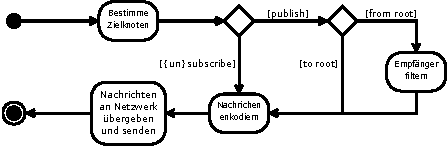
\includegraphics{grafics/processing_send.pdf}}
\caption{Versand von Nachrichten}
\label{fig:processing_send}
\end{figure}

Werden Nachrichten in forward behandelt, müssen diese erst dekodiert werden, wie es in \Fref{fig:processing_forward} aufgezeigt ist. Die Verteilungs- und Filterpolicies können anhand der Verwaltungsinformationen ihren Zustand anpassen und wenn nötig die Nachricht ändern oder gar stoppen.

\begin{figure}[htbp]
\centering
\resizebox{\textwidth}{!}{%

\includegraphics{grafics/processing_forward.pdf}}
\caption{Verarbeitung von Nachrichten in forward}
\label{fig:processing_forward}
\end{figure}

Die Abarbeitung der Nachrichten in deliver ist komplexer als die beiden oben genannten Fälle, da hier alle Policies zusammenarbeiten wie in \Fref[plain]{fig:processing_deliver} dargestellt. Nach der Entschlüsselung werden Subscribe- und Unsubscribe-Nachrichten ähnlich wie bei der Behandlung in forward verarbeitet. Die Policies können ihren Zustand aktualisieren.\\
Publish-Nachrichten müssen eine Validitätsprüfung bestehen, bevor entschieden wird, ob sie eine Nachricht \emph{to root}, also an die Rootknoten sind, oder nicht. Jeder Rootknoten und alle anderen Knoten auf dem Verteilungsweg, die selbst Verteilungsaufgaben übernehmen müssen (abhängig von der gewählten Verteilungspolicy), leiten nun das Verteilen der Nachricht ein. Dazu wird in einem ersten Schritt eine neue Publishnachricht \emph{from root} erstellt, alle Verwaltungsinformationen abgefragt und schließlich die Nachricht mit dem obig beschriebenen Verfahren gesendet. Nun wird an diesen Knoten geprüft ob sie selbst an diesem Kanal angemeldet sind und, falls dies zutrifft, ob sie an der Nachricht interessiert sind. Wenn nicht, endet die Bearbeitung der Nachricht. Ansonsten trifft sich der Ablaufpfad an dieser Stelle mit dem Ablaufpfad einfacher Knoten, die lediglich Subscriber sind. Die Synchronisierungspolicy ermöglicht eine Wohlordnung der Nachricht und kann diese sowohl komplett zurückhalten als auch mehrere Nachrichten zurückgeben, falls durch die aktuelle Nachricht weitere Nachrichten ``freigeschaltet'' werden. Alle Nachrichten werden nun nochmals auf ihre Validität geprüft, da zurückgehaltene Nachrichten inzwischen veraltet sein können. Für jede valide Nachricht wird eine Signalisierung der Zustellung laut Policy, zum Beispiel eine Bestätigungsnachricht zurück an den Sender, ermöglicht. Bevor die Nachrichten schließlich an die Applikation übergeben werden, können sie persistiert werden.

\begin{figure}[htbp]
\centering
\resizebox{\textwidth}{!}{%
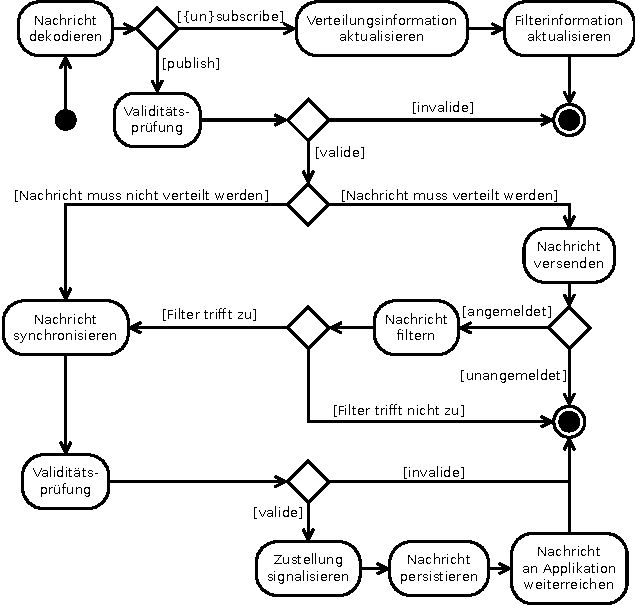
\includegraphics{grafics/processing_deliver.pdf}}
\caption{Verarbeitung von Nachrichten in deliver}
\label{fig:processing_deliver}
\end{figure}

Der nächste Abschnitt prüft das eingeführte Verarbeitungsmodell anhand einiger Strategien auf seine Tauglichkeit. Dazu werden hauptsächlich Verteilungsstrategien genutzt, da diese die Hauptarbeit im System tragen.

\subsection*{Beispielhafte Strategien}
Für jede einzelne Policy bietet \ac{m2etis} mehrere konkrete Implementierungen an und lässt sich mit benutzerdefinierten Strategien weiter auf die Anforderungen der Applikation anpassen\footnote{siehe \Fref{fig:metis_aufbau}}. In diesem Kapitel wird das Verarbeitungsmodell anhand zweier Verteilungsalgorithmen getestet. Scribe \cite{Castro2002Scribe} erzeugt wie beschrieben einen Multicast-Tree, während der andere Algorithmus an VON \cite{Hu2006VON} angelehnt ist und seinen Fokus auf die ``in-game''-Nachbarschaft legt. Dies ist vor Allem auf Events mit einer hohen Lokalität sinnvoll. Der Einfluss solcher Events, wie zum Beispiel Positionsänderungen, wirkt sich nur in einem begrenzten Gebiet aus und muss daher nur benachbarten Knoten -- im Spiel -- mitgeteilt werden.

Zuerst wird das Verarbeitungsmodell zum Nachrichtenversand und danach der Empfang und die Verteilung von Nachrichten betrachtet.

Bei Scribe richten sich im Gegensatz zu VON die Zielknoten nach der Nachrichtenart und dem Typ des Knotens. Subscribe- und Unsubscribe-Nachrichten, wie auch Publish-Nachrichten normaler Knoten, werden immer an den Rootknoten des Channels gesendet. Hierzu kann der Hashwert des Kanalnamens berechnet und auf einen Schlüssel im Netz abgebildet werden. Verteilt der Rootknoten oder weitere Knoten auf dem Verteilungsweg eine Publish-Nachricht so gibt Scribe die Lister der an diesme Knoten eingeschriebenen Subscriber zurück.\\
Ein Algorithmus wie VON kann auf Applikationswissen zugreifen und liefert als Empfänger einer Subscribe-Nachricht die Nachbarn im Spiel sind zurück. Diese Nachbarschaftmetrik muss sich nicht alleine auf die Position im Spiel beziehen, sondern kann auch von der Mitgliedschaft in Gruppen bestimmt werden; sie ist aber in jedem Falle spezifisch für den gewählten Eventtyp. Unsubscribe-Nachrichten richten sich prinzipell an die gleichen Nachbarn -- jedoch müssen diese mit den Nachbarn zur Anmeldung abgeglichen werden. Publish-Nachrichten zur werden zuerst immer an den Knoten selbst geschickt, damit dieser in der Abarbeitung in deliver den Event an alle eingetragenen Empfänger senden kann.

Scribe verarbeitet Subscribe- und Unsubscribe-Nachrichten in forward. Jeder Knoten auf dem Routingpfad vom Sender zum Rootknoten fügt den Sender der Nachricht seiner Liste der Empfänger hinzu und ändert die Anmeldenachricht: Er trägt sich als Absender ein. Der Multicast-Tree wird also Knoten für Knoten beim Routing der Nachrichten aufgebaut. Sollte der Knoten schon angemeldet sein, kann er die Nachricht terminieren und damit effektiv die Anzahl an Nachrichten begrenzen.\\
Die von Scribe geforderte periodische Auffrischung der Anmeldung erfolgt für normal angemeldete Knoten außerhalb der Verteilungsstrategie: Die Anmeldung wird nach einem, von der Strategie bestimmten Zeitintervall, wiederholt. Ist ein Knoten aufgrund seiner Lage im Multicast-Tree angemeldet, kann er diese Anmeldung auffrischen, wenn periodische Anmeldungen zu bearbeiten sind. Hierbei ist es wichtig, dass die Filterstrategie bei allen Auffrischungen involviert ist, damit die Prädikate weiterhin im Baum zusammengeführt werden. Durch die periodischen Anmeldungen werden auch ausgefallene Knoten ausgetauscht, denn die Nachrichten werden vom Netzwerk über andere Knoten geroutet und somit wird der Multicast-Tree wieder aufgebaut.\\
Der VON-ähnliche Algorithmus bearbeitet alle Nachrichten in deliver. Der Sender der Subscribe-Nachricht wird in die Liste der Empfänger eingetragen. Eine Publish-Nachricht wird an all diese weitergeleitet. Da ein Knoten nicht bei sich selbst angemeldet ist, kann die Bearbeitung der Nachricht beendet werden.

Es ist allerdings auch möglich eine Verteilungsstratege wie VON gänzlich anders zu implementieren. Alle Anmeldungen für sind lediglich implizit und werden nicht als Nachrichten auf das Netzwerk gelegt. Statt eine Publish-Nachricht an den eigenen Knoten zu senden, wird diese allen Nachbarn im Spiel zugestellt. Dies bedeutet, dass Publish-Nachrichten vom Sender mit \emph{from root} statt \emph{to root} markiert werden.\\
Mit diesem implizitem System entfällt auch die Abmeldung am Kanal.

Diese drei vorgestellen Implementierungsansätze verschiedender Verteilungsstrategien zeigt wie mächtig das Verarbeitungsmodell ist und welchen Spielraum es verschiedenen Strategien bietet um Events anhand der angebotenen Dimensionen bestmöglich zu bearbeiten.
